%!TEX root = ../masters_thesis.tex

% basic idea: given initial state $t_0$, consecutively insert Hivent Operations changing this state
% current state: accumulate all changes

\chapter{Introduction} % (fold)
\label{cha:introduction}
\begin{large}
\begin{quoteit}
  Imagine there's no countries \\
  It isn't hard to do \\
  Nothing to kill or die for \\
  And no religion too \\
  Imagine all the people \\
  Living life in peace
\end{quoteit}
\end{large}
\hfill \textit{-- John Lennon, \emph{Imagine} (1971)}

The song of John Lennon is an anthem for peace on Earth, for brotherhood of people, for the end of materialism -- but also for the end of countries. He connects the concept of a country to nationalism that encourages people to fight and die for. John Lennon wrote the song in the 1970s, in the midst of the Cold War between the capitalistic and the socialistic bloc, only 30 years after World War II and 50 years after World War I. Especially in Europe this time point would have probably not been described as ``peaceful''. And not just John Lennon connected this lack of peace with the existance of national states divided by artificial borders.

Now, another 45 years later, the situation in Europe looks much different: Most countries are united in a confederation of a largly shared economy. While there are still countries with clearly defined borders, they are mostly of legal nature, but citizens of the European Union can travel freely within large parts of Europe. This concept is celebrated as a major achievement, but it is mostly forgotten that the concept of nations with solid borders has not been there 200 years ago. While travelling back then was probably not as pleasent as it is today, Goethe at least did not need a passport when he travelled to Italy and back to Weimar. He also did not travel not from country ``Germany'' via ``Austria'' to ``Italy'', but he rather crossed several duchies and principalities that do not exist anymore.

% ==============================================================================
\section{Motivation} % (fold)
\label{sec:motivation}

What we might call ``our country'' today has changed a lot in the past. Hardly any of the current 193 member states of the United Nations is in its same border as 100 years ago. The countries have evolved in time and space. Would it not be nice to see this development? On a map that shows the state of the world at an arbitrary point in history? So that we can see how our country looked like 100 years ago? 200 years ago? 1000 years ago? How settelements became cities and principalities became national states? While there are many historical sources describing one point in history, may it be governmental bills, historical maps or diary entries of kings, there is no such thing as a comprehensive historical world atlas that lets you travel back in time and space and explore \emph{when} our country changed, \emph{where} it changed -- and most importantly \emph{why}? This thesis is all about that: How can the historical development of countries be shown, for the benefit of a better understanding of how we became what we are today.

This is a very complicated undertaking, given that countries have changed frequently. But there are even more severe problems: How do we know how a country has looked like in 1600? And if we find an historical map of this time, can we trust it? How certain can we be that the countries and their borders are true? The next problem is that the history of countries can also be contradictory. There is not always \emph{one story} which is supported by all sides. There are contested territories, even today, from which it is not clear who they belong to. There are ``places'', even today, which are not clearly a ``country'' because some might disagree. There is a whole lot of uncertainty and diagreement in the history of countries that this thesis deals with.

Finally, the state of the world can not be visualized at any point in history just like this -- because there is no freely available dataset. It is not just a visualization problem, it is a data problem. And to go even further: It is a data model problem because it is not even straightforward to say what kind of information is actually necessary to show the history of countries. And if we have found a data model and found some data, nobody wants to write it into a database table. Another goal for this thesis is to develop a well-designed user interface to edit the history of countries directly on the map.

% section motivation (end)

% ==============================================================================
\section{Problem Domain} % (fold)
\label{sec:problem_domain}

\begin{quoteit}
  All human actions takes and makes place. \\
  The past is the set of places made by human action. \\
  History is a map of these places. \\
  The past thus exists not in time but in space.
\end{quoteit}
\hfill -- Philip J. Ethington in \cite[précis]{citeTakeMakePlace}

\emph{Time} and \emph{space} are everywhere. They are highly related to our lives and the objects we perceive. The temporal perception of the world is driven by events, may they be personal life events like a wedding or world events like the end of World War II. While a point in time can be described by a date and a time stamp, it is not always easy to scale and grasp. This is mainly because some temporal developments happen suddenly, like a natural disaster, and some happen very slowly throughout years, decades or even centuries, like climate change. Time is not tangible. For space, the situation is different, because it can be perceived as physically existing: A place is just there, we can go there and see it. Each point on this planet can be exactly described by a pair of geographic coordinates and a combination of them can describe a line or an area.

The combination of both concepts in one information system would allow to say how something has developed in space over time. \emph{Geographic Information Systems} (GIS) model, acquire, manage, analyze and visualize data with a spatial relation to the Earth, mostly on a map. Most GIS answer two basic questions about an object: \emph{Where} it is in relative or absolute location and \emph{what} it is, being its attributes or properties. As an example, a country is expressed by a set of borders consisting of border points in geographic coordinates and by meta-information like its name or its population. However, most of the current GIS are limited to the spatial dimension. They can not answer to the question \emph{when} a country was found or how its borders have developed in the previous fifty years. For that purpose \textbf{\emph{Historical Geographic Information Systems}} (HGIS) were developed. They extend general GIS with the dimension of time.

There are several \emph{spatio-temporal data models} to model the temporal development of spatial objects. The straightforward approach immediately derives from the the concept of historical maps: At certain time points a \emph{snapshot} is taken: a map showing the current state at this point in time. Snapshots can immediately answer the question how the the world has looked like at this date. However, they fail to answer the next question: What has changed since last time, when and why? Given two historical maps of Germany, one at 1871 after the formation of the German Empire and one 1919 after the Treaty of Versailles -- how did it look like at the beginning of World War I in 1914?

\begin{figure}[H]
  \centering
  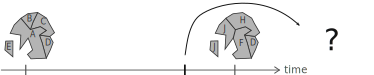
\includegraphics[width=0.8\textwidth]{graphics/introduction/snapshot_approach}
  \caption{The snapshot approach for modelling time and space}
  \label{fig:snapshot_approach}
\end{figure}

As it is seen in figure \ref{fig:snapshot_approach}, this is impossible to say, because there is no information about an arbitrary time point between two snapshots! Also, if the map only shows Germany and its neighboring countries, what about Russia, Sub-Saharan Africa or South East Asia? For an interactive historical world atlas, the snapshot approach is neither suitable nor feasible, because it requires a whole new world map every time some country changes on Earth.

The key problem is that snapshots can not say what has changed, because they do not store changes. This is the approach of another class of spatio-temporal data models: \emph{Event-based} models. They store two things: one reference snapshot and a set of events that happen at a certain time point and trigger changes on the map relative to the last event.

\begin{figure}[H]
  \centering
  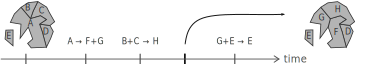
\includegraphics[width=0.8\textwidth]{graphics/introduction/event_based_approach}
  \caption{The event-based approach for modelling time and space}
  \label{fig:event_based_approach}
\end{figure}

Figure \ref{fig:event_based_approach} shows an example of an event-based approach. There are three changes that consecutively happen to the snapshot on the left. The question how the world looked like at an arbitrary point in time can be answered like this: It is the state of the reference map and all the changes of all events since that time point accumulated. In the case of figure \ref{fig:event_based_approach}, country $A$ split up into $F$ and $G$ and $B$ and $C$ have unified to $H$. This approach is suitable for modelling a countries history, because each change to the state of a country was introduced by some histoircal event, may it be a declaration or a peace treaty.

% ------------------------------------------------------------------------------
\paragraph{Research Questions} % (fold)
\label{par:research_questions}

The goal of this thesis is to lay a theoretical foundation for an information system that deals with the development of countries in time and space. The domain is limited to countries, their names and their borders and historical events that change them. In addition to the theory, an open-source Web-based prototype is to be developed. It should provide a well-designed user interface for editing historical data about countries allowing the user to directly manipulate the countries on the map. For that matter there are three research questions to be answered throughout the thesis:

\begin{enumerate}
  \item What type of historical changes can happen in the development of countries in time and space?
  \item How can these changes be
  \begin{enumerate}
    \item modeled in an information system?
    \item edited by humans in a user interface?
  \end{enumerate}
  \item How can the model handle uncertainty and disagreement in history?
\end{enumerate}

% paragraph research_questions (end)

% ==============================================================================
\newpage
\section{Overview} % (fold)
\label{sec:overview}

The following part of the thesis is structured in four chapters. The second chapter introduces the basic concepts of the problem domain: First of all the suprisingly difficult concept of a \emph{country} is introduced in section \ref{sec:countries}. Afterwards the term \emph{Historical Geographic Information Systems} is clarified in section \ref{sec:historical_geographic_information_systems}), followed by state of the art of \emph{spatio-temporal data models} (\ref{sec:spatio_temporal_data_models}). The last section \ref{sec:histoglobe} presents the application that the model developed in this thesis will be implemented in: \emph{HistoGlobe}.

Chapter 3 is the main chapter of this thesis. It describes the development process of this thesis and answeres the first two research questions: The \emph{Hivent Model} in section \ref{sec:hivent_model} introduces a set of five \emph{Hivent Operations} that can model all possible changes to the development of countries in time and space. The next section \ref{sec:editing_hivent_data} presents approaches to edit data in the Hivent Model using \emph{Edit Operations}, a different set of operations that is well-understood by humans. The interface for the information system of this thesis was developed using a \emph{Human-Centered Design} approach. The process and the result of it is illustrated in section \ref{sec:user_interface_design_process}. The chapter closes in \ref{sec:application} with an insight into the implementation of the data model and the user interface in the HistoGlobe application.

extensions
first briefly evaluate the data model, edit methods, interface and system as a whole.
develop extensions dealing with uncertainty and disagreement.

summary of the results
outsight into the future: possible extensions

% section overview (end)

% ==============================================================================

% chapter introduction (end)